\documentclass[11pt]{report}
\usepackage{adjustbox}
\usepackage{xcolor}
\usepackage{gensymb}

\topmargin=0.0in %length of margin at the top of the page (1 inch added by default)
\oddsidemargin=0.0in %length of margin on sides for odd pages
\evensidemargin=0in %length of margin on sides for even pages
\textwidth=6.5in %How wide you want your text to be
\marginparwidth=0.5in
\headheight=0pt %1in margins at top and bottom (1 inch is added to this value by default)
\headsep=0pt %Increase to increase white space in between headers and the top of the page
\textheight=9.0in



\begin{document}

%%%%%%%%%%%%%%%%%%%%%%%%%%%%%%%%%%%%%%%%%%%%%%%%%%%%%%%%%%%%%%%%%%%%%%%%%%%%
\begin{titlepage}
\begin{center}
\textsc{\LARGE University of Pittsburgh}\\[1.5cm]
{\huge \bfseries STEPUP Image Analysis User Guide\\[0.4cm] }

\begin{figure}[!h]
\begin{center}
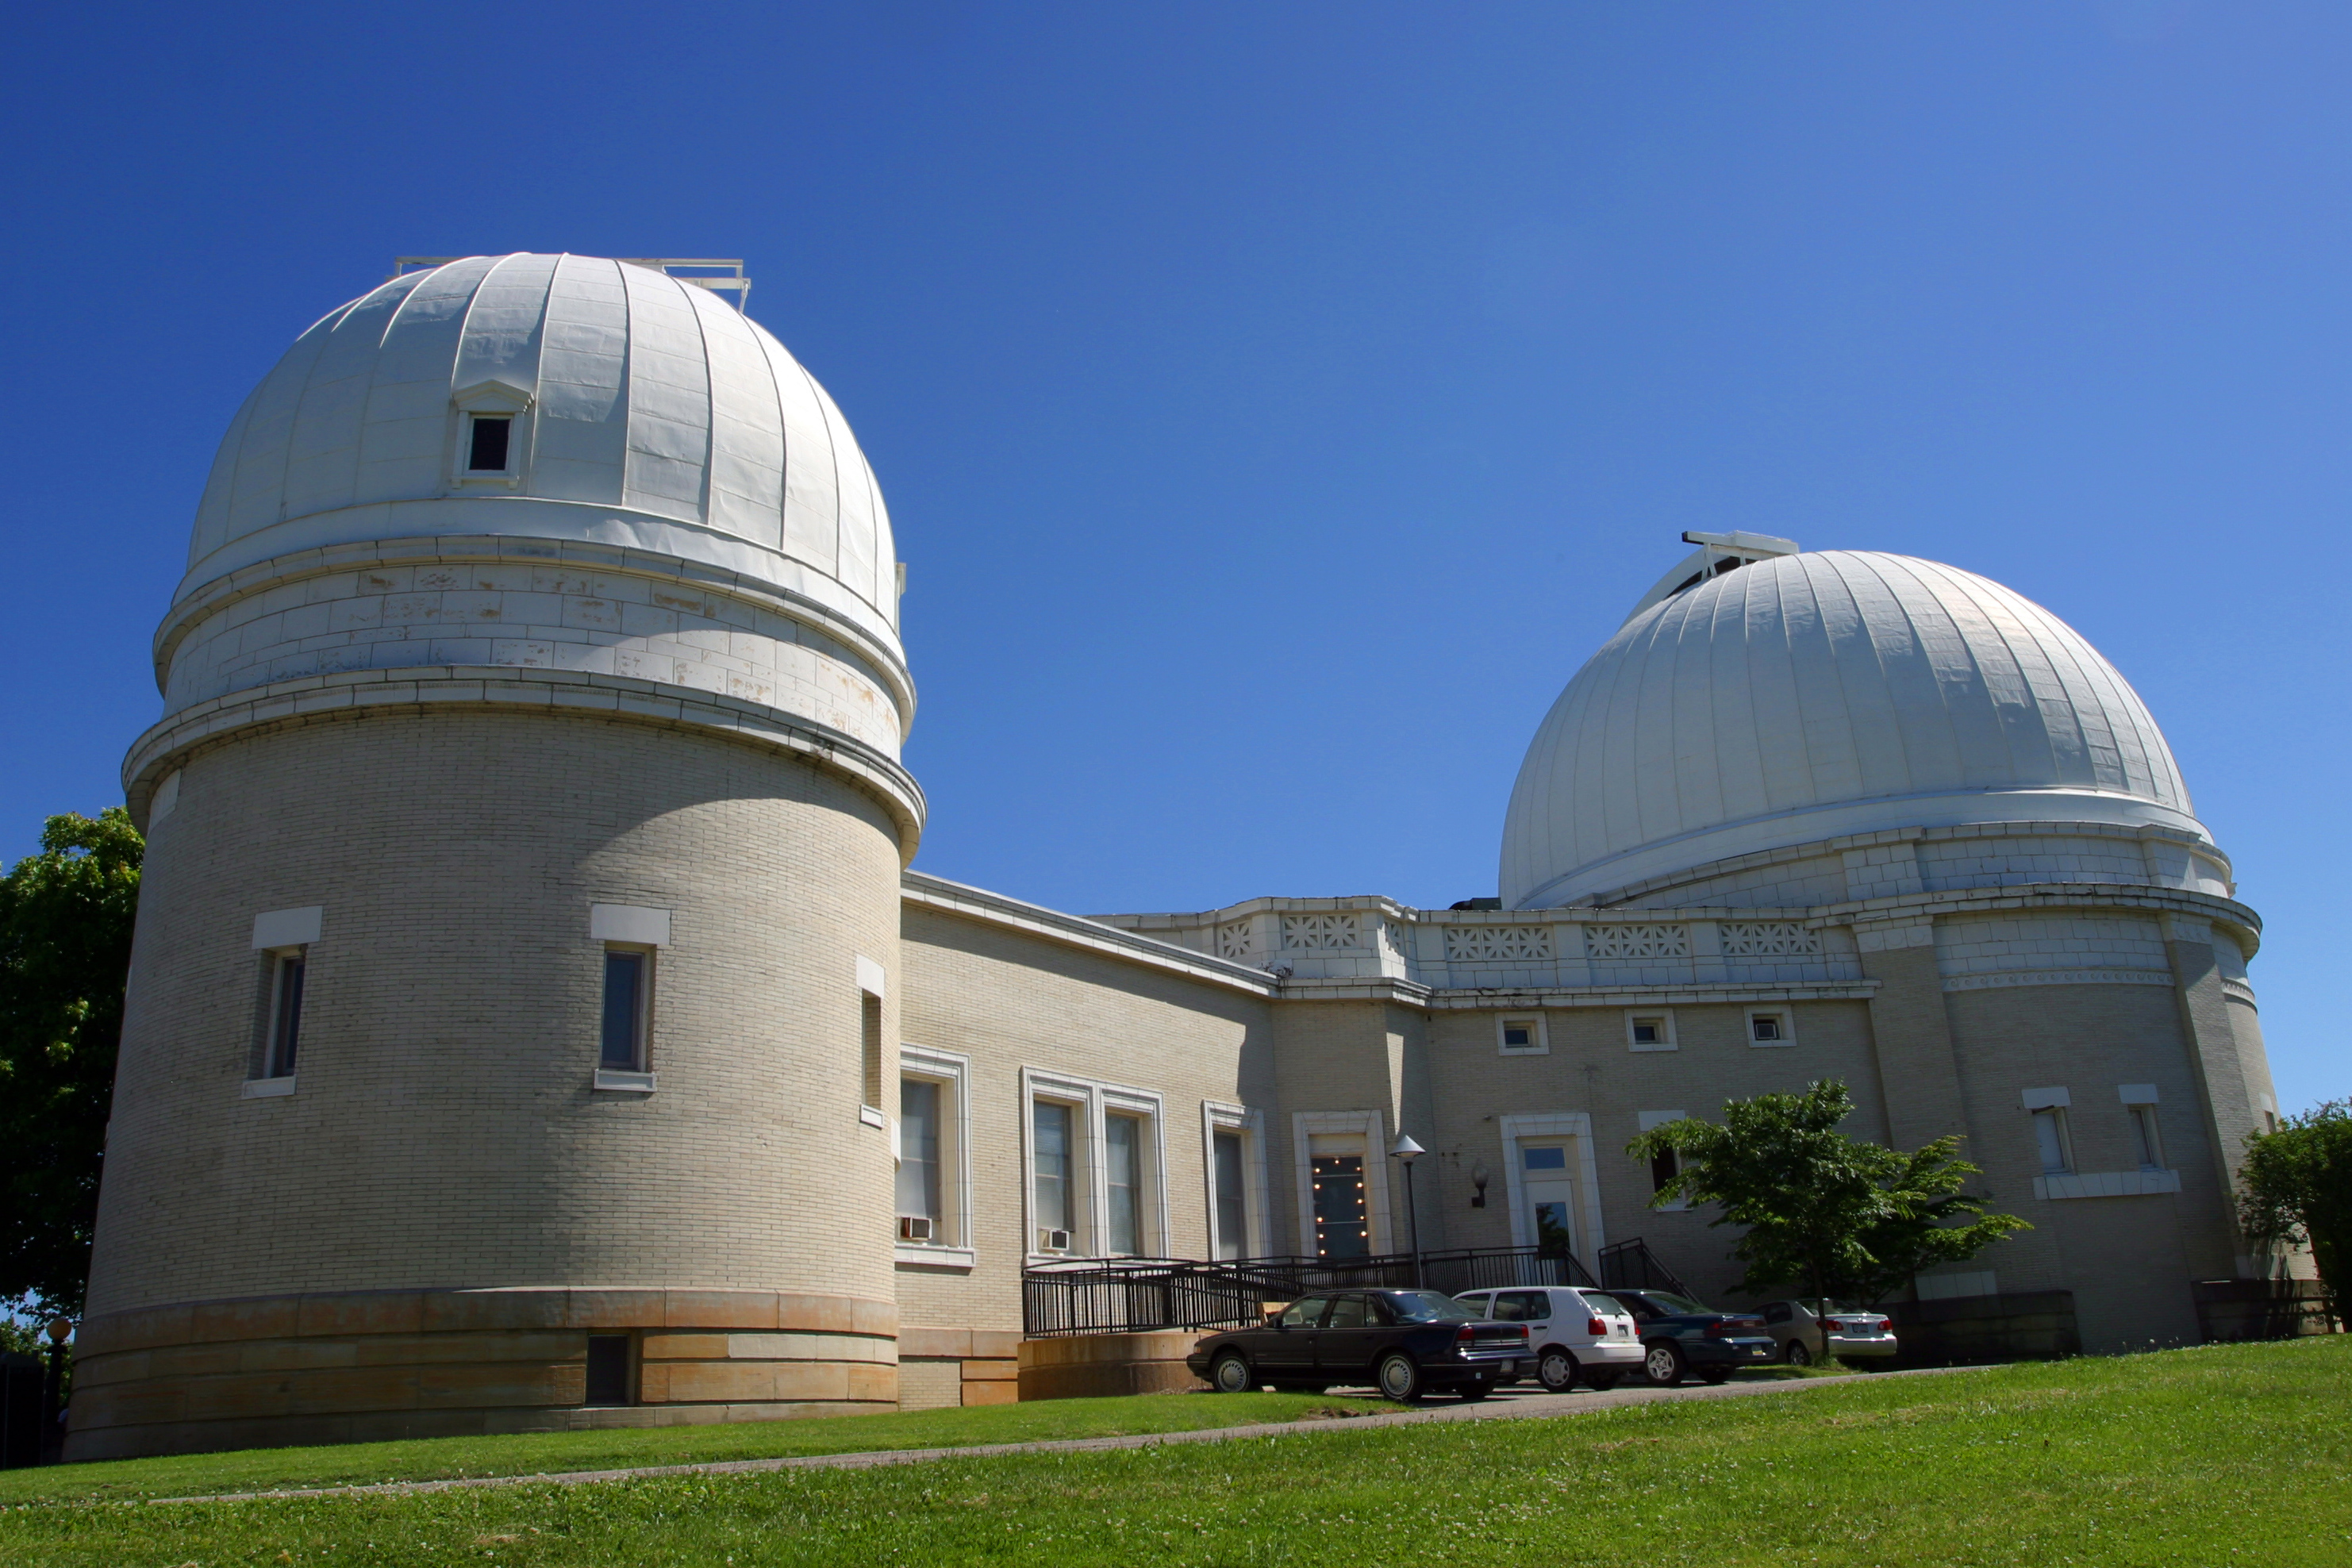
\includegraphics[totalheight=.5\textheight]{Title.jpg}
\end{center}
\begin{center}
\emph{Allegheny Observatory}
\end{center}
\end{figure}

\vfill
\begin{minipage}{0.4\textwidth}
\begin{flushleft}\large
\emph{Author:}\d\
Helena Richie
\end{flushleft}
\end{minipage}
\begin{minipage}{0.4\textwidth}
\begin{flushright} \large
\emph{Supervisor:} \\
Professor Wood-Vasey
\end{flushright}
\end{minipage}

\end{center}
\end{titlepage}
%%%%%%%%%%%%%%%%%%%%%%%%%%%%%%%%%%%%%%%%%%%%%%%%%%%%%%%%%%%%%%%%%%%%%%%%%%%%
\tableofcontents
\chapter{Preliminary Steps}

\section{Transferring Data}

\begin{enumerate}
\item Begin by checking to see if a directory has already been made for the night of observation that you wish to run the code on. Do this by typing: {\bf cd /home/depot/STEPUP/raw/\emph{target-name}}. If the directory for your target does not exist, use the {\bf mkdir} command to make a directory for your target in {\bf /home/depot/STEPUP/raw}. Either way, the last command you type should be {\bf mkdir /home/depot/STEPUP/raw/\emph{target-name}/\emph{date-of-observation}}. 
\item Once there is a directory for your night of observation, use the {\bf cd} command to enter it. Now, in order to access the data on the observatory computer, type {\bf ftp aoserver1.univ.pitt.edu}. When it prompts you for a name, type \emph{anonymous}. You may type anything for the password and hit enter.
\item Now you must go to the directory from which you wish to transfer data. Do this by typing {\bf cd /STEPUPDataFiles/\emph{date-of-observation}}.
\ Before you begin copying files, make sure that prompting is turned off so that you do not have to confirm the transfer of each file individually. Do this by typing {\bf prompt}. The setting toggles between on and off, so you may need to type it twice to make sure it says that prompting is turned off.
\item Next, type {\bf binary}. This changes the mode to transfer.
\item Finally, to copy the files use the {\bf mget} command. Type {\bf mget \emph{name-of-target}*.fit}. This will transfer all files that have the target name in the title and the ".fit" extension. If you do not have a copy of the observing report on the Astro Lab computers, be sure to type {\bf mget obsreport.txt} to transfer it as well. 
\item Type {\bf bye} to log off of the observatory computer.
\end{enumerate}

\section{Creating Input File}
Note: As a rule of thumb, the formatting of each parameter in the input file should match previous formatting of the same parameter in other cases. For example, the \emph{date} parameter should always be formatted as \emph{YYYY-MM-DD}. Also, when you see the angle brackets "$\langle$" and "$\rangle$", you should know to replace the general formatting with your specific information in the correct formatting inside of the brackets. For example, if you're creating an input file for the night of August 19th, 2017 and see {\bf $\langle$YYYY-MM-DD$\rangle$}, you should know to replace it with {\bf 2017-09-19}. Also, be sure to use both capital and lowercase letters as appropriate.
\begin{enumerate}
\item Copy the input file template to the target directory by typing {\bf cp /home/depot/STEPUP/} {\bf raw/input-file.txt /home/depot/STEPUP/raw/\emph{target-name}/\emph{date-of-observation}}. 
\item Make sure you are {\bf cd}'ed into the night's directory and type the command {\bf gedit input-file.txt}. Now you will begin editing the file.
\item Go through the file and input all of the parameters that you're immediately aware of. These should include {\bf DATE, TARGET, RA} and {\bf DEC}. If you are unsure of any of them, check the observing report.
\item Now that you have completed all of the immediately known entries, you must determine {\bf VSPCODE, COMPMAGS, COMPCOORDS, CNAME, CCOORDS, KNAME} and {\bf KCOORDS}. All of this information will be found on \emph{aavso.org}. Go to that site and sign in. 
\item Once you are on the site and logged in, mouse over the \emph{Observing} tab at the top. Under the \emph{Variable Star Charts} option, click on \emph{Variable Star Plotter (VSP)}. 
\item Once on the Variable Star Plotter page, you will need to specify the right ascension, declination, predefined chart scale (which should be option F, 18.5 arcminutes), and the filters which the photometry table should display (at the bottom). If you have previously used VSP for this target, you may skip these steps and simply use the Chart ID from last time, which can be found in the input-file.txt for that night of observing. Once you have filled out this information, click \emph{Plot Chart} at the bottom. {\bf Note:} It is important that you check that all of the stars given in the photometry table are {\bf entirely} in the image. If they are not, be sure not to include any of the information for that star in the input-file.txt, as it will cause an error in the program if you do. 
\item You should have been redirected to a page that has a star chart for your target on it. At the top under where it says "Variable Star Plotter" click \emph{Photometry Table for This Chart}.
\item Back in input-file.txt, enter the bolded code at the top where it says "Report this sequence as..." in the {\bf VSPCODE} entry point.
\item Now, in the {\bf COMPMAGS} category, enter in the magnitudes in the order that they appear, top to bottom, each separated by a comma. \textbf{Important}: be sure to include the magnitude values for only the filter that you observed in.
\item Also in order from top to bottom, enter the right ascension and declination for each comparison star under the {\bf COMPRA} and {\bf COMPDEC} keywords. They should be in the form {\bf HH:MM:SS} for RA and {\bf DD:MM:SS} for Dec.
\item Now you will need to choose one "comparison" star and one "check" star that the program will output data on. Choose the two of the closest stars in the image to the target star by looking at the numerical values of the RA and Dec and comparing them to that of the target star. These will be your comparison star and check star (it doesn't matter which is which). Enter in their AAVSO Unique Identifier (AUID), RA, and Dec into the {\bf CLABEL, CRA, CDEC, KLABEL, KRA}, and {\bf KDEC} categories. 
\item Now that you have completed all of the entries, verify that the file is in your target directory by {\bf cd}ing into your target directory and then using the {\bf ls} command, which will show you everything in the current directory you are in. It should be saved in the directory exactly as \emph{input-file.txt}. If it is named anything other than that, be sure to change it. 
\begin{figure}[!h]
\begin{center}
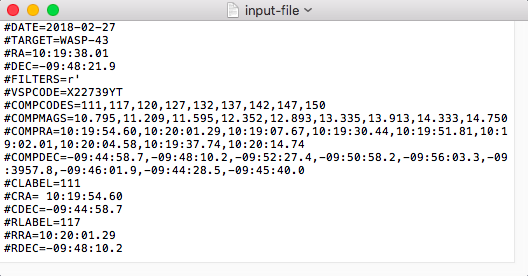
\includegraphics[totalheight=.3\textheight]{example.png}
\end{center}
\begin{center}
\small{Example of input-file.txt}
\end{center}
\end{figure}
\end{enumerate}

\chapter{Running STEPUP Image Analysis}
\begin{enumerate}
\item Before you run the code, be sure to check that you have all of the calibration and target images in your directory as well as that your input file. Additionally, make sure that the naming of each image is consistent with the target name that you put in your input file and how your directory is named.
\item Now, open a new terminal window and type {\bf cd home/depot/STEPUP/STEPUPImageAnalysis/}. Now that you have entered into the directory containing the code, type the command {\bf python3 main.py}. This will begin running the code.
\item You will first be prompted for the name of the target. Be consistent as you enter it and be sure not to include any additional capital/lowercase letters and spaces.
\item Next, you will be prompted to enter the date of observation. Enter is as {\bf YYYY-MM-DD} with no additional spaces.
\item Now the instrument signature removal part of the program should be running. When it is finished, the program will pause as it asks you if you would like the rest of the program to continue running or end with instrument signature removal. If you would like the rest of the program to run, enter accordingly, but first you must create an image of the field of view of the target star with WCS information in its header before the program starts running again.\
\item To generate this image, go to \emph{astrometry.net}
\item Once on their homepage, select the \emph{use} option. 
\item Now on the \emph{Use the Code} page, select \emph{web}.
\item At the top of the page you're redirected to, select \emph{Upload}. You will go into the directory that was just created containing all of your instrument signature removed images. It should be called {\bf /home/depot/STEPUP/raw/\emph{name-of-target}/\emph{date-of-observation}/ISR\_Images/}. Choose any one of the images in there.
\item Once you have chosen your image, select \emph{Upload}. It will take a minute or so for the image to upload, so don't press anything of leave the page until it does.
\item You will be redirected to a new page. It will take another minute or so for the image to be processed. Once it says \emph{Success}. Click on \emph{Go to results page}.
\item Under the \emph{Calibration} column along the right side, click on \emph{new-image.fits}. This will save the image to the computer's {\bf Downloads} directory.
\item Move this image into the directory with your instrument signature removed images by typing {\bf mv /home/Downloads/new-image.fits /home/depot/STEPUP/raw/\emph{name-of-target}/\emph{date-of-observation}/ISR\_Images/}. Now that this image is the correct directory, enter {\bf Y} to continue.
\item If you continued with the program, the astrometry part of the program will begin to run. This takes may take up to an hour to complete, so keep checking in on the program every 15 minutes or so as it runs. Once this part is completed, the program will ask if you would like it to perform photometry. Answer as needed.
\item After the photometry process has completed the program will be finished running. Check your target directory to make sure that a \emph{lightcurve.pdf} and a \emph{output.txt} file are both in there. Also open up the files and check to make sure they look okay. If anything seems out of the ordinary, see the troubleshooting section to determine any possible errors.
\end{enumerate}

\chapter{Uploading Data}
\begin{enumerate}
\item Once you have ran the program on your dataset and have your \emph{output.txt} file, go to \emph{www.aavso.org}.
\item On the AAVSO homepage, under the \emph{Observing} tab, select \emph{WebObs (Search AID or Submit Your Data)}.
\item On the \emph{WebObs} page, select \emph{Upload a file of observations}.
\item Now, on the \emph{Upload a File of Observations} page, click \emph{Choose File} and find your \emph{output.txt} file in your target directory and select it.
\item Now that you have selected the file, click \emph{Upload File}.
\end{enumerate}

%%%%%%%%%%%%%%%%%%%%%%%%%%%%%%%%%%%%%%%%%%%%%%%%%%%%%%%%%%%%%%%%%%%%%%%%%%%%
\end{document}